\begin{figure}[H]
\centering
\includegraphics[page=6,width=0.48\textwidth]{\FCNCFigures/xTFW/showFake_sideband/reg2mtau1b2jos_vetobtagwp70_highmet/tau_pt_0.pdf}
\put(-100, 140){\textbf{(a1)}}
%\put(-120, 130){\footnotesize{$t_h\thadhad$-2j (OS)}}
\includegraphics[page=6,width=0.48\textwidth]{\FCNCFigures/xTFW/showFake_sideband/reg2mtau1b3jos_vetobtagwp70_highmet/tau_pt_0.pdf}
\put(-100, 140){\textbf{(b1)}}
%\put(-120, 130){\footnotesize{$t_h\thadhad$-3j (OS)}}
\caption{  The distributions of $\tau$ $\pt$ in the $t_h\thadhad$-2j (a1), $t_h\thadhad$-3j (b1) using the OS CR derived FFs. Only statistical uncertainties are being shown. Underflow and overflow bins are included respectively in the first and last bins. Empty data bins here are always blinded based on our strategy.}
\label{fig:fakeEstimation_had_oscr}
\end{figure}

